%%%%%%%%%%%%%%%%%%%%%%%%%%%%%%%%%%%%%%%%%%%%%%%%%%%%%%%%%%%%%%%%%%%%%%%%%%%%%%%%
%%
%% CT Lab Notes
%% Copyright (C) 2017  Joshua Ellis
%% Department of Physics
%% The University of Melbourne
%%
%%%%%%%%%%%%%%%%%%%%%%%%%%%%%%%%%%%%%%%%%%%%%%%%%%%%%%%%%%%%%%%%%%%%%%%%%%%%%%%%

%%%%%%%%%%%%%%%%%%%%%%%%%%%%%%%%%%%%%%%%%%%%%%%%%%%%%%%%%%%%%%%%%%%%%%%%%%%%%%%%
%% HEADER
%%%%%%%%%%%%%%%%%%%%%%%%%%%%%%%%%%%%%%%%%%%%%%%%%%%%%%%%%%%%%%%%%%%%%%%%%%%%%%%%

%% In general, LaTeX commands start with `\` and consist of letters only.
%% Optional parameters are specified in brackets `[]`, whilst compulsory
%% arguments (if any) are specified in braces `{}`.  (Strictly speaking, this is
%% only a convention and packages can use other things.  One notable example is
%% the Beamer package which adds extra optional arguments with `<>'.)
%%
%% LaTeX is generally insensitive to whitespaces including newlines.  So if a
%% functions takes a lot of arguments or has many options, it can be easily
%% split across lines without repercussions.  The one important exception is
%% that full empty lines mark the end/start of a paragraph.

%% All LaTeX documents begin with the the `\documentclass` command which serves
%% to set the general style of the document.  It defines the page layout, the
%% chapter/section styles, how figures appear, etc. and may provide some
%% additional environments too.  LaTeX comes with four main classes: `article`,
%% `report`, `book` and `letter`.
%%
%% The [KOMA-script](https://www.ctan.org/pkg/koma-script) package provides
%% alternatives to replacements for the default classes (`scrartcl`, `scrreprt`,
%% `scrbook`, `scrlttr2`) and provides a lot of options to more easily customize the
%% layout of the page.
\documentclass[
  a4paper,             % The size of the layout
  11pt,                % The font size (10pt, 11pt, 12pt)
  oneside,             % Whether the document is one-sided or two-sided
  onecolumn,           % Whether to have one or two columns in the layout
  bibliography=totoc,  % Adjust how the bibliography appears in ToC
  final,               % As opposed to draft (which speeds up compilation)
]{scrartcl}
%% Note all of these optional arguments are required; in fact, most of the ones
%% specified here would have been chosen by default if left unspecified.  There
%% are also some other options which have not be specified but they are
%% documented in the [KOMA-script](https://www.ctan.org/pkg/koma-script)
%% documentation.
%%
%% One of the important options in the list above is `draft`/`final`.  If draft
%% mode is enabled, LaTeX and most packages will disable features which take up
%% a lot of time in order to speed up compilation.  Draft mode also highlights
%% certain error in the output document.  On the other hand, final mode enables
%% all features which will increase (sometimes quite significantly) the
%% compilation time of the document.

%% The part of the document starting from here through to the `\begin{document}`
%% command is called the preamble.  This is where you include additional
%% packages which provide additional functionalities.  Below are many packages
%% which I use on a semi-regular basis.
%%
%% Although you'll find that they are all enabled below, this is for the sake of
%% checking compatibility between all the packages.  It is advisable to only
%% enable those packages you actually need as this will speed up compilation,
%% and decrease the likelihood that two packages conflict.
%%
%% All packages are available from the Comprehence TeX Archive Network (CTAN) at
%% http://ctan.org.  Quite often, for each `\usepackage{pkg-name}`, it is
%% possible to go to http://ctan.org/pkg/pkg-name in order to find information
%% about the package (there are a few exception to this though, in which case a
%% Google search will suffice).
%%
%% Although you'll know the reason for including a package initially, most
%% people will forget this initial reason after a few months.  It is a **VERY**
%% good idea to have a small comment next to *EVERY* `\usepackage` giving a
%% quick recap as to what this package does.  This will be invaluable in case
%% you include two packages which conflict each other.

%% For the vast majority of packages, the order in which they are loaded does
%% not matter.  There are a few exceptions though, mostly relating to the
%% various referencing packages (hyperef, cleveref, ...).  The following package
%% must be loaded first and provides some additional functionalities to other
%% packages.
\usepackage{ifluatex}  % Provides the command \ifluatex

%% Formatting
%%%%%%%%%%%%%%%%%%%%%%%%%%%%%%%%%%%%%%%%%%%%%%%%%%%%%%%%%%%%%%%%%%%%%%%%%%%%%%%%

\usepackage{geometry}   % Customize text width, page height, margins, etc.
\geometry{
  %% See the geometry package's documentation for all the options available
  textwidth=13cm,
}

\usepackage{pageslts}   % Improved page numbering
\usepackage{enumitem}   % Easily customize lists

%% Change the formatting of titles and sections.
\setkomafont{part}{\normalfont\scshape\Huge}
\setkomafont{partnumber}{\normalfont\scshape\huge}
\setkomafont{section}{\normalfont\Huge}
\setkomafont{subsection}{\normalfont\huge}
\setkomafont{subsubsection}{\normalfont\Large}
\setkomafont{paragraph}{\normalfont\large\scshape}

%% Change the formatting of section entries in the table of contents
\setkomafont{sectionentry}{\scshape}

%% Modify the indentation at the start of each paragraph.
\setlength\parindent{1em}
\setlength\parskip{0.3\baselineskip plus 0.5\baselineskip minus 0.1\baselineskip}

%% Font
%%%%%%%%%%%%%%%%%%%%%%%%%%%%%%%%%%%%%%%%%%%%%%%%%%%%%%%%%%%%%%%%%%%%%%%%%%%%%%%%

\usepackage{microtype}   % Fine small typographical details
\usepackage{realscripts} % Use the font's sub- and superscripts

%% LaTeX allows for some if-else statements.  It is very rare that you'll have
%% to use them, though this is one example since we only want to include a
%% particular package if this example is compiled with LuaLaTeX.
\ifluatex
  \usepackage{fontspec}  % Allows for any font to be specified

  % Change the main font
  \setmainfont{EB Garamond}[
    Contextuals={Alternate},
    Ligatures={Common,Contextual,Rare,TeX},
    Numbers=OldStyle,
    % CharacterVariant={1},    % historical s
    % CharacterVariant={3},    % historical j
    % CharacterVariant={6},    % guillemets
    % CharacterVariant={11},   % distinguish i and 1
    % CharacterVariant={21},   % a
    % CharacterVariant={27},   % g
    ItalicFeatures={
      CharacterVariant={4},  % &
      CharacterVariant={5:3},  % v
    }
  ]

  % Change the mono-space font
  \setmonofont{Fira Code}[
    Scale=MatchLowercase,
  ]
\else
  \usepackage{ebgaramond}  % A fall-back that isn't as nice as fontspec
\fi %% marks the end of the if-else statement

\usepackage[cmintegrals,varg]{newtxmath}  % Nice math font with Garamond

%% Languages
%%%%%%%%%%%%%%%%%%%%%%%%%%%%%%%%%%%%%%%%%%%%%%%%%%%%%%%%%%%%%%%%%%%%%%%%%%%%%%%%

\usepackage[UKenglish]{babel}           % Set up the language
\usepackage[style=british]{csquotes}    % Advanced handling of quotes
\usepackage[perpage]{footmisc}          % Count per-page

%% siunitx is an incredible useful package to display numbers and their
%% associated units.  It also offers extra commands to specify lists and ranges
%% of values with units.  Some commands which it provides include:
%% - \SI{quantity}{units}
%% - \SIRange{start}{end}{units}
%% - \SIList{a, b, ..., d}{units}
%% With the units being given as `\kilo\metre\per\year\per\pico\barn`.
\usepackage{siunitx}

%% Adjust the way units are displayed in ranges and units so that they are only
%% mentinoed once.
\sisetup{
  range-units=single,
  list-units=single,
}

%% Graphics & Figure
%%%%%%%%%%%%%%%%%%%%%%%%%%%%%%%%%%%%%%%%%%%%%%%%%%%%%%%%%%%%%%%%%%%%%%%%%%%%%%%%

%% Graphics can be included in a LaTeX document with
%%
%% ```
%% \includegraphics[options]{image}
%% ```
%%
%% Usually, the extension for the image is not specified and LaTeX will
%% figure out the best one.  It is of course possible to add the extension to
%% specify a particular image.
%%
%% In order to ensure that the image is a particular width, you can use
%% `width=<distance>`.  This will also scale the height but keep the aspect
%% ratio (if you also specify the height, the aspect ratio will not be kept).
%% It is tempting to specify an exact distance such as `4cm`; but it is
%% generally better to have a relative distance such as `0.4\linewidth`.  This
%% way, the image will scale nicely if the context is changed.
\usepackage{graphicx}   % Handle graphics

%% Look for images in the './images/' sub-directory
\graphicspath{{./images/}}

\usepackage{xcolor}     % Define and use colours
\usepackage{subcaption} % Subfigures inside a figure

\usepackage{tikz}       % Powerful drawing language
\usepackage{pgfplots}   % Plotting with LaTeX
\pgfplotsset{compat=1.15}

\pgfplotsset{
  % Silently ignore missing points
  unbounded coords=discard,
  % filter discard warning=false,
  % Alter the default axis style so that minor ticks are used and a
  % corresponding grid as well.
  every axis/.append style={
    minor tick num=3,
    grid=both,
    major grid style={
      color=black,
      opacity=0.1,
    },
    minor grid style={
      color=black,
      opacity=0.05,
    },
  },
  % Add the cousins of the Viridis colormap
  colormap/magma/.style={%
    /pgfplots/colormap={magma}{%
      rgb=(0.001462, 0.000466, 0.013866)
      rgb=(0.035520, 0.028397, 0.125209)
      rgb=(0.102815, 0.063010, 0.257854)
      rgb=(0.191460, 0.064818, 0.396152)
      rgb=(0.291366, 0.064553, 0.475462)
      rgb=(0.384299, 0.097855, 0.501002)
      rgb=(0.475780, 0.134577, 0.507921)
      rgb=(0.569172, 0.167454, 0.504105)
      rgb=(0.664915, 0.198075, 0.488836)
      rgb=(0.761077, 0.231214, 0.460162)
      rgb=(0.852126, 0.276106, 0.418573)
      rgb=(0.925937, 0.346844, 0.374959)
      rgb=(0.969680, 0.446936, 0.360311)
      rgb=(0.989363, 0.557873, 0.391671)
      rgb=(0.996580, 0.668256, 0.456192)
      rgb=(0.996727, 0.776795, 0.541039)
      rgb=(0.992440, 0.884330, 0.640099)
      rgb=(0.987053, 0.991438, 0.749504)
    },
  },
  colormap/inferno/.style={%
    /pgfplots/colormap={inferno}{%
      rgb=(0.001462, 0.000466, 0.013866)
      rgb=(0.037668, 0.025921, 0.132232)
      rgb=(0.116656, 0.047574, 0.272321)
      rgb=(0.217949, 0.036615, 0.383522)
      rgb=(0.316282, 0.053490, 0.425116)
      rgb=(0.410113, 0.087896, 0.433098)
      rgb=(0.503493, 0.121575, 0.423356)
      rgb=(0.596940, 0.154848, 0.398125)
      rgb=(0.688653, 0.192239, 0.357603)
      rgb=(0.775059, 0.239667, 0.303526)
      rgb=(0.851384, 0.302260, 0.239636)
      rgb=(0.912966, 0.381636, 0.169755)
      rgb=(0.956852, 0.475356, 0.094695)
      rgb=(0.981895, 0.579392, 0.026250)
      rgb=(0.987464, 0.690366, 0.079990)
      rgb=(0.973088, 0.805409, 0.216877)
      rgb=(0.947594, 0.917399, 0.410665)
      rgb=(0.988362, 0.998364, 0.644924)
    },
  },
  colormap/plasma/.style={%
    /pgfplots/colormap={plasma}{%
      rgb=(0.050383, 0.029803, 0.527975)
      rgb=(0.186213, 0.018803, 0.587228)
      rgb=(0.287076, 0.010855, 0.627295)
      rgb=(0.381047, 0.001814, 0.653068)
      rgb=(0.471457, 0.005678, 0.659897)
      rgb=(0.557243, 0.047331, 0.643443)
      rgb=(0.636008, 0.112092, 0.605205)
      rgb=(0.706178, 0.178437, 0.553657)
      rgb=(0.768090, 0.244817, 0.498465)
      rgb=(0.823132, 0.311261, 0.444806)
      rgb=(0.872303, 0.378774, 0.393355)
      rgb=(0.915471, 0.448807, 0.342890)
      rgb=(0.951344, 0.522850, 0.292275)
      rgb=(0.977856, 0.602051, 0.241387)
      rgb=(0.992541, 0.687030, 0.192170)
      rgb=(0.992505, 0.777967, 0.152855)
      rgb=(0.974443, 0.874622, 0.144061)
      rgb=(0.940015, 0.975158, 0.131326)
    },
  },
  colormap/jpeBlWhBl/.style={%
    /pgfplots/colormap={jpeReWhBl}{%
      rgb=(0.094957, 0.211745, 0.949475)
      rgb=(0.149676, 0.288182, 0.889340)
      rgb=(0.210373, 0.340936, 0.846637)
      rgb=(0.268241, 0.383971, 0.815988)
      rgb=(0.322709, 0.422216, 0.794156)
      rgb=(0.374335, 0.457967, 0.779078)
      rgb=(0.423724, 0.492464, 0.769388)
      rgb=(0.471369, 0.526452, 0.764155)
      rgb=(0.517653, 0.560415, 0.762732)
      rgb=(0.562866, 0.594688, 0.764671)
      rgb=(0.607234, 0.629520, 0.769662)
      rgb=(0.650934, 0.665108, 0.777508)
      rgb=(0.694107, 0.701609, 0.788103)
      rgb=(0.736875, 0.739156, 0.801431)
      rgb=(0.779363, 0.777851, 0.817590)
      rgb=(0.821732, 0.817752, 0.836891)
      rgb=(0.863910, 0.858922, 0.860421)
      rgb=(0.902313, 0.903243, 0.885111)
      rgb=(0.879049, 0.855058, 0.839087)
      rgb=(0.860371, 0.806330, 0.794603)
      rgb=(0.843643, 0.758010, 0.750027)
      rgb=(0.828754, 0.709912, 0.704933)
      rgb=(0.815142, 0.662021, 0.659169)
      rgb=(0.802302, 0.614305, 0.612550)
      rgb=(0.789774, 0.566724, 0.564903)
      rgb=(0.777122, 0.519227, 0.516091)
      rgb=(0.763930, 0.471751, 0.466024)
      rgb=(0.749803, 0.424208, 0.414668)
      rgb=(0.734369, 0.376470, 0.362052)
      rgb=(0.717286, 0.328322, 0.308250)
      rgb=(0.698243, 0.279394, 0.253349)
      rgb=(0.676967, 0.228987, 0.197339)
      rgb=(0.653216, 0.175627, 0.139788)
      rgb=(0.626782, 0.115406, 0.078551)
      rgb=(0.597480, 0.029268, 0.008874)
    },
  },
  colormap/jpeWhRe/.style={%
    /pgfplots/colormap={jpeWhRe}{%
      rgb=(0.902313, 0.903243, 0.885111)
      rgb=(0.879049, 0.855058, 0.839087)
      rgb=(0.860371, 0.806330, 0.794603)
      rgb=(0.843643, 0.758010, 0.750027)
      rgb=(0.828754, 0.709912, 0.704933)
      rgb=(0.815142, 0.662021, 0.659169)
      rgb=(0.802302, 0.614305, 0.612550)
      rgb=(0.789774, 0.566724, 0.564903)
      rgb=(0.777122, 0.519227, 0.516091)
      rgb=(0.763930, 0.471751, 0.466024)
      rgb=(0.749803, 0.424208, 0.414668)
      rgb=(0.734369, 0.376470, 0.362052)
      rgb=(0.717286, 0.328322, 0.308250)
      rgb=(0.698243, 0.279394, 0.253349)
      rgb=(0.676967, 0.228987, 0.197339)
      rgb=(0.653216, 0.175627, 0.139788)
      rgb=(0.626782, 0.115406, 0.078551)
      rgb=(0.597480, 0.029268, 0.008874)
    },
  },
  % Set Viridis as the default colormap
  colormap/viridis,
}

% \endinput

\usetikzlibrary{
  angles,
  calc,
  quotes,
  shadings,
}

%% TikZ pictures and plots can significantly increase the time it takes to
%% produce the output.  The `external` TikZ library library defers the creation
%% of these figures to a sub-process which creates a separate PDF file which is
%% then simply imported into the main document.  To call the sub-process, you
%% have to execute the appropriate makefile.  If you are using LatexMk, you can
%% use the `.latexmkrc` to automatically do this for you.
%%
%% The following setup works on Linux, and should work on OS X too.
\usetikzlibrary{external}
\tikzexternalize[shell escape=-shell-escape, prefix=images/tikz/]
\immediate\write18{mkdir -p images/tikz/}
\tikzset{
    external/mode=list and make,
    external/system call={
        lualatex \tikzexternalcheckshellescape -halt-on-error -interaction=batchmode -jobname="\image" "\texsource" || rm "\image.pdf"},
}

%% Math Packages
%%%%%%%%%%%%%%%%%%%%%%%%%%%%%%%%%%%%%%%%%%%%%%%%%%%%%%%%%%%%%%%%%%%%%%%%%%%%%%%%

\usepackage{amsmath}     % The core math package
\usepackage{amssymb}     % Defines additional math fonts and symbols
\usepackage{mathtools}   % Various extra maths functions
\usepackage{dsfont}      % A double stroke font (for double stroke 1)

%% Define a new command called \withnumber which forces the line to have number
%% (even if it is referenced elsewhere).
\newcommand\withnumber{\refstepcounter{equation}\tag{\theequation}}

%% Allows page breaks in math (1 = avoid if possible, 4 = whenever).  Page
%% breaks can be avoided at particular places by using \\* instead of \\.
\allowdisplaybreaks[2]

%% Only number referenced equations
\mathtoolsset{showonlyrefs}

%% Code
%%%%%%%%%%%%%%%%%%%%%%%%%%%%%%%%%%%%%%%%%%%%%%%%%%%%%%%%%%%%%%%%%%%%%%%%%%%%%%%%

\usepackage{minted}

%% Define \texinline
\newmintinline[texinline]{latex}{}

%% Define \rawinline
\newmintinline[rawinline]{text}{}

%% Linking and Referencing
%%%%%%%%%%%%%%%%%%%%%%%%%%%%%%%%%%%%%%%%%%%%%%%%%%%%%%%%%%%%%%%%%%%%%%%%%%%%%%%%

\usepackage{hyperref}  % Automatically inserts hyperlinks.
\usepackage{cleveref}  % Use `\cref` to reference anything

%% Define some slightly nicer colors
\definecolor{link-color}{RGB}{96 0 0}
\definecolor{cite-color}{RGB}{0 96 0}
\definecolor{file-color}{RGB}{0 0 96}
\definecolor{url-color}{RGB}{0 0 96}
\definecolor{link-border-color}{RGB}{255 159 159}
\definecolor{cite-border-color}{RGB}{159 255 159}
\definecolor{file-border-color}{RGB}{159 159 255}
\definecolor{url-border-color}{RGB}{159 159 255}

\hypersetup{
  %% When `colorlinks` is true, all links will be coloured which looks nice in
  %% digital version of the document but not in print.  If the document is
  %% intended for printing, then `colorlinks` should set to false.
  colorlinks=true,
  linkcolor=link-color,
  citecolor=cite-color,
  filecolor=file-color,
  urlcolor=url-color,
  linkbordercolor=link-border-color,
  citebordercolor=cite-border-color,
  urlbordercolor=url-border-color,
}

%% Glossary
%%%%%%%%%%%%%%%%%%%%%%%%%%%%%%%%%%%%%%%%%%%%%%%%%%%%%%%%%%%%%%%%%%%%%%%%%%%%%%%%
%% This package requires `makeglossaries` to be run after the initial run of
%% LaTeX so that the glossary is generated and the a second run of LaTeX is need
%% to included the newly generated glossary.  (This is automatically handled by
%% Latexmk with the provided .latexmkrc).

%% hyperref should be loaded first
\usepackage[toc]{glossaries}
\usepackage{glossaries-extra}

\setglossarystyle{index}
\setabbreviationstyle[acronym]{long-short-sc}

\loadglsentries{glossary.glos}

% \makeglossaries

%% Bibliography
%%%%%%%%%%%%%%%%%%%%%%%%%%%%%%%%%%%%%%%%%%%%%%%%%%%%%%%%%%%%%%%%%%%%%%%%%%%%%%%%

%% hyperref should be loaded first
\usepackage[
  %% See the extensive documentation for biblatex for a description of what
  %% these options do
  autocite=inline,
  backend=biber,
  biblabel=brackets,
  doi=true,
  eprint=true,
  maxnames=4,
  style=phys,
]{biblatex}

%% Add a bib file
\addbibresource{references.bib}

%% Other modifications/package
%%%%%%%%%%%%%%%%%%%%%%%%%%%%%%%%%%%%%%%%%%%%%%%%%%%%%%%%%%%%%%%%%%%%%%%%%%%%%%%%

\usepackage{jpellis}

%% Define a Fourier transform operator
\DeclareMathOperator{\FT}{\scrF}

%% Question
%%%%%%%%%%%%%%%%%%%%%%%%%%%%%%%%%%%%%%%%%%%%%%%%%%%%%%%%%%%%%%%%%%%%%%%%%%%%%%%%

\usepackage{tcolorbox}
\tcbuselibrary{breakable}


% \usepackage{framed}

\newcounter{question}
\newenvironment{question}{%
  \stepcounter{question}%
  \begin{tcolorbox}[
      colframe=black,
      sharp corners=all,
      boxsep=0.5ex,
    ]
    \noindent\textsc{\large Question \arabic{question}:} %
}{%
  \end{tcolorbox}%
}

%% Document Information
%%%%%%%%%%%%%%%%%%%%%%%%%%%%%%%%%%%%%%%%%%%%%%%%%%%%%%%%%%%%%%%%%%%%%%%%%%%%%%%%

%% Define a few shorthand commands.  The `makeatletter' and `makeatother' allows
%% the use of '@' in commands which is reserved for hidden functions.
\makeatletter
\newcommand\@department{}
\newcommand\department[1]{\renewcommand\@department{#1}}

\newcommand\@university{}
\newcommand\university[1]{\renewcommand\@university{#1}}

\newcommand\@keywords{}
\newcommand\keywords[1]{\renewcommand\@keywords{#1}}

\AtEndPreamble{
  %% Set the PDF metadata, though this can only be done once they've been all
  %% defined which is at the end of the preamble.
  \hypersetup{
    pdftitle={\@title},
    pdfauthor={\@author},
    pdfsubject={\@subject},
    pdfkeywords={\@keywords},
  }
}
\makeatother

%% The \texorpdfstring string will, depending on context, either print proper
%% TeX command (in this case LaTeX will the special kerning), or the plain text
%% fallback.  This is useful if you have equation, links or special formatting
%% in titles as the PDF bookmarks can't handle them.
\title{Computed Tomography Lab}
\subtitle{\texorpdfstring{
    \textsc{phyc30021} -- Laboratory and Computational Physics 3
  }{
    PHYC30021 -- Laboratory and Computational Physics 3
  }
}

\subject{Computed Tomography Lab}
\keywords{lab notes, computed tomography}

\author{Joshua P.~\textsc{Ellis}}
\department{School of Physics}
\university{The University of Melbourne}

\date{\today}

%%%%%%%%%%%%%%%%%%%%%%%%%%%%%%%%%%%%%%%%%%%%%%%%%%%%%%%%%%%%%%%%%%%%%%%%%%%%%%%%
%% DOCUMENT
%%%%%%%%%%%%%%%%%%%%%%%%%%%%%%%%%%%%%%%%%%%%%%%%%%%%%%%%%%%%%%%%%%%%%%%%%%%%%%%%
\begin{document}
%% Adjust the pagenumbering to capital Latin letters
\pagenumbering{Alph}

%% Title
%%%%%%%%%%%%%%%%%%%%%%%%%%%%%%%%%%%%%%%%%%%%%%%%%%%%%%%%%%%%%%%%%%%%%%%%%%%%%%%%
%% We don't want any page numbers, chapter headings, etc. on the page
\pagestyle{empty}

\begin{titlepage}
  \makeatletter
  \begin{center}
    \vspace*{2.5cm}
    {\Huge \@title}
    \vskip0pt
    \rule{\linewidth}{2pt}
    \vskip0pt
    {\Large \@subtitle}
    \vskip\fill
    
\includegraphics[width=0.3\paperwidth]{unimelb}
    \vskip\fill
    {\Large By \@author}
    \vskip0.5em
    {\Large \@department}
    \vskip2em
    {\large \@date}
  \end{center}

\makeatother
\end{titlepage}

%% Table of Content
%%%%%%%%%%%%%%%%%%%%%%%%%%%%%%%%%%%%%%%%%%%%%%%%%%%%%%%%%%%%%%%%%%%%%%%%%%%%%%%%
\cleardoublepage
\pagestyle{plain}
\pagenumbering{roman}

\tableofcontents

%%%%%%%%%%%%%%%%%%%%%%%%%%%%%%%%%%%%%%%%%%%%%%%%%%%%%%%%%%%%%%%%%%%%%%%%%%%%%%%%
%% CONTENT
%%%%%%%%%%%%%%%%%%%%%%%%%%%%%%%%%%%%%%%%%%%%%%%%%%%%%%%%%%%%%%%%%%%%%%%%%%%%%%%%
\cleardoublepage
\pagestyle{headings}
\pagenumbering{arabic}

\section{Introduction}
\label{sec:introduction}

In 1895, Wilhelm R\"ontgen systematically studied a new form of radiation which,
to everyone's great surprise, was able to penetrate through soft tissue but was
mostly stopped by bones.\footnote{He was not the first to discover X-rays, nor
  was he the first to notice that they were able to penetrate through certain
  materials; however, he was the first to systematically study
  them.}~\cite{rontgen96a,rontgen96b,rontgen97,rontgen96_translation} Up until
that point, the only way to see inside a person was during surgery or using a
cadaver; this new possibility of imaging the inside of a patient without
requiring surgery was revolutionary.  In what is now one of the first medical
images, R\"ontgen created a radiograph of his wife's left hand
(\cref{subfig:first_x-ray}) and since then, medical imaging has improved greatly
(\cref{subfig:modern_x-ray}) and it is regularly used in hospitals.

\begin{figure}
  \centering
  \begin{subfigure}{0.39\linewidth}
    \centering
    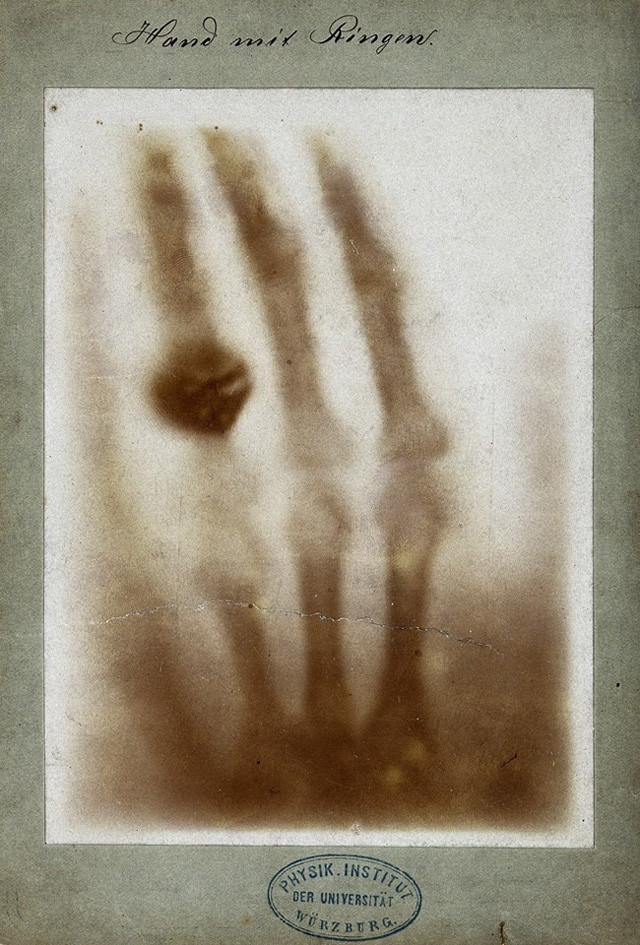
\includegraphics[width=0.9\linewidth]{first_x-ray}
    \caption{One of the first medical X-ray image.  Taken by Wilhelm R\"ontgen of
      his wife's left hand. }
    \label{subfig:first_x-ray}
  \end{subfigure}
  \begin{subfigure}{0.59\linewidth}
    \centering
    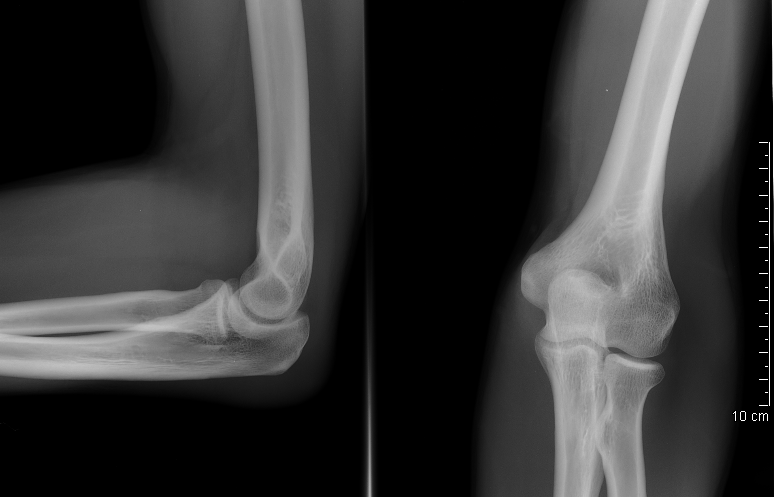
\includegraphics[width=0.9\linewidth]{modern_x-ray}
    \caption{A modern X-ray image of an elbow.}
    \label{subfig:modern_x-ray}
  \end{subfigure}
  \caption{X-ray images.}
  \label{fig:x-rays}
\end{figure}

One disadvantage of X-ray images such as those in \cref{fig:x-rays} is that an
opaque object will obstruct everything in front and behind it.  In the case of
bones this is may not be too much of an issue as there aren't many overlapping
bones in the human body and the patient and/or radiograph can be rotated to
ensure the desired region isn't obstructed.  On the other hand, this may not be
possible when imagine soft tissue such as in a radiograph of the abdomen.  In
order to see what might be in front or behind the opaque object, the X-ray
projection has to be taken from a different angle, but the question then
becomes:
\begin{displayquote}
  Given a set of X-ray images from different angles, can we reconstruct the full
  \textsc{3d} shape of the original object?
\end{displayquote}
As you might expect, the answer is \emph{yes} and is exactly what happens in
\gls{CT} scans.  The process of reconstructing the full \textsc{3d} object from
these different projection angles is called \emph{tomographic reconstruction}
and will be the focus of this lab.

Although the term \enquote{\gls{CT} scans} is now synonymous with X-ray \gls{CT}
scans, it is possible to use kinds of radiation.  Some example well-known
examples in the medical field include \gls{PET} and \gls{MRI} scans.  Even
outside the medical field, \gls{CT} scans are used in many other fields from
geophysics to atmospheric science to astrophysics.

\subsection{Aim}
\label{subsec:aim}

In this lab, the mathematical properties of tomographic projection and
reconstruction will first be investigated.  An algorithm to numerically project
images will be implemented, replicating what happens when an X-ray image is
taken.  Subsequently, the original image will be reconstructed from the
projected image using back-projection and filtered back-projection.

Once these algorithms are implemented, the effects of other effects that can
arise in realistic scenarios can be investigated.  This section of the lab is
intended to be exploratory and is open-ended.  It will be up to the student to
decide what they wish to investigate.  Some ideas that may be investigated
include:
\begin{itemize}
\item The effects of noise during the creation of projection and its effect on
  the reconstruction;
\item The effects of defects in the detector such as a dead/malfunctioning
  pixel;
\item Limitations in the angles that can be projected and how that can affect
  the quality of the reconstructed image;
\item Limitations in the resolution of the detector and how that can affect the
  quality of the reconstructed image.
\end{itemize}
This list is not exhaustive and other aspects can also be explored.  It is not
necessary to answer \emph{all} questions and they are mostly there to help.

\cleardoublepage
\section{Projections and Reconstructions}
\label{sec:projections_and_reconstructions}

Before anything can be implemented, the processes involved in creating X-ray
projections and subsequently reconstructing the original image from the
projections must be understood.  In the case of the former process, a simple
physical understanding of attenuation is sufficient.  As for the latter process,
it is much less obvious and the mathematical properties of these properties were
first investigated by Johann Karl August Radon (16 December 1887--25 May 1956)
\cite{radon17,radon86_translation}.

\subsection{Projections}
\label{subsec:projections}

X-rays are capable of penetrating through materials and they generally either
travel in straight lines, or get absorbed by the material.  How strongly they
get absorbed depends on the composition of the material which, in general, will
vary as a function of position.

For an infinitesimal segment \(\dd \eta\), the attenuation coefficient \(\mu\)
is given by
\begin{equation}
  \label{eq:attenuation_def}
  \mu = - \frac{1}{I} \ddfrac{I}{\eta},
\end{equation}
where \(I\) is the intensity of the X-ray.  In the special case where the
material has a constant attenuation factor over some distance \(d\), the overall
attenuation factor is
\begin{equation}
  I = I_{0} e^{-\mu d}.
\end{equation}
In general though, the attenuation factor depends on many other factors and will
vary in space (and possibly even time, though we'll ignore this here); thus,
over the full path of the X-ray, the total attenuation is obtained by
integrating \cref{eq:attenuation_def}:
\begin{equation}
  \label{eq:attenuation}
  I = I_{0} \exp\left[ - \int \mu(x, y) \dd \eta \right].
\end{equation}

When an X-ray image of an object is taken, a projection of the object density is
being created along a particular direction.  Consider the diagram in
\cref{fig:projection} with the \((x, y)\) coordinates provide a fixed reference
coordinate system.  The X-rays are coming from particular direction and, by
assumption, they are all parallel.  It is convenient to define the \((\xi,
\eta)\) coordinates such that \(\eta\) is parallel to the X-ray, and \(\xi\) is
perpendicular to the ray.

From \cref{eq:attenuation}, it becomes clear that we can now define the overall
attenuation along an X-ray path, or \emph{projected attenuation}, as:
\begin{equation}
  \label{eq:projected_attenuation}
  p_{\theta}(\xi) = \ln\left( \frac{I}{I_{0}} \right) = - \int \mu(x, y) \dd \eta
\end{equation}
where \(x\) and \(y\) are implicitly functions of \(\xi\) and \(\eta\) (see
\cref{fig:projection}).

The projected attenuation is, ultimately, function of \(\theta\) and \(\xi\) as
the integration is done over all \(\eta\).  In a sense, we can think of
\(p_{\theta}(\xi)\) as a polar function, though unlike a true polar function,
\(\xi\) is allowed to be negative and \(\theta\) goes over the range \([0,
\pi)\).

\begin{figure}
  \centering
  \begin{tikzpicture}
    %% The main shape.  Define an overall radius
    \def\R{1.5}
    \shade [
        smooth,
        opacity=0.4,
        upper left=red,
        upper right=blue!40!white,
        % lower left=red!40!white,
        lower right=blue]
      plot [
        domain=-3.142:3.142,
        samples=501,
        parametric,
        id=object]
      function{
        \R * (sin(t) + 0.2*sin(2*t) + 0.1*cos(2*t)),
        \R * (cos(t) + 0.3*cos(3*t) + 0.2*sin(4*t))
      };

    %% Add the original axis
    \draw [-stealth] (-2*\R, 0) -- (2*\R, 0)
      node [pos=1, anchor=west] {\(x\)};
    \draw [-stealth] (0, -2*\R) -- (0, 2*\R)
      node [pos=1, anchor=south] {\(y\)};

    %% Define a rotated coordinates
    \def\rot{25}
    \pgfmathsetmacro\sinrot{sin(\rot)}
    \pgfmathsetmacro\cosrot{cos(\rot)}

    %% Draw the angle
    \coordinate (x)  at (1, 0);
    \coordinate (O)  at (0, 0);
    \coordinate (xi) at (\cosrot, \sinrot);
    % \draw [red, thick] (x) -- (O) -- (xi);
    \draw (x) -- (O) -- (xi)
          pic [draw, thick, angle eccentricity=1.1, angle radius=1.3*\R cm, "\(\theta\)"]
          {angle = x--O--xi};

    \begin{scope}[rotate=\rot]
      \draw [-stealth] (-2*\R, 0) -- (2*\R, 0)
        node [pos=1, anchor=west] {\(\xi\)};
      \draw [-stealth] (0, -2*\R) -- (0, 2*\R)
        node [pos=1, anchor=south] {\(\eta\)};

      \foreach \i in {-2, -1.6, ..., 2} {
        \draw [-stealth, black!40!white] (\i, 1.6*\R) -- (\i, -1.6*\R);
      }

      \draw [thick] (-2.2, -1.6*\R) -- (2.2, -1.6*\R)
         node [sloped, below, pos=0.7] {\(p_{\theta}(\xi)\)};
      \foreach \i in {-2.1, -2.0, ..., 2.21} {
        \draw [thin] (\i - 0.1, -1.6*\R - 0.1) -- (\i, -1.6*\R);
      }
    \end{scope}
  \end{tikzpicture}
  \caption{Diagram illustrating the path travelled by X-rays.  The X-rays are
    travelling along the \(\eta\) direction and being projected on the surface
    (photographic plate or detector) on the bottom right.}
  \label{fig:projection}
\end{figure}

This integral along perpendicular lines is called \emph{Radon transform}, named
after the Austrian mathematician Johann Radon and the function
\(p_{\theta}(\xi)\) is called the \emph{sinogram} of \(\mu\).  In this lab, the
Radon transform of \(\mu(x, y)\) will be denoted by \(p_{\theta}(\xi)\), but
more generally the Radon transform of some function \(f(x, y)\) is denoted as
\(\calR_{x,y}\{ f(x, y) \}(\theta, \xi)\) in analogy to the way Fourier
transforms are denoted.\footnote{If the variables being transformed are obvious
  from context, the Radon transform is simply written as \(\calR f\).}

\begin{question}
  Why is \(p_{\theta}(\xi)\) called a sinogram?  (Hint: plot it)
\end{question}

\begin{question}
  Show that the Radon transform is linear and distributive.  That is
  \begin{equation}
    \calR(a f + b g) = a \calR f + b \calR g
  \end{equation}
  for any functions \(f\) and \(g\), and scalars \(a\) and \(b\).
\end{question}

\begin{question}
  Calculate analytically the Radon transform for the function
  \begin{equation}
    f(x, y) =
    \begin{cases}
      1 & x^{2} + y^{2} \leq R^{2} \\
      0 & \text{otherwise}
    \end{cases}
  \end{equation}
\end{question}

\subsection{Tomographic Reconstruction}
\label{subsec:tomographic_reconstruction}

In practice, \(\mu(x, y)\) can't be measured directly without taking apart the
object; however, it is possible to pass X-rays through the unknown object and
\(p_{\theta}(\xi)\) for a range of \(\xi\) and \(\theta\) values.  The intent is
to now reconstruct the original function \(\mu(x, y)\) based on the measured
\(p_{\theta}(\xi)\) values.

This section will make use of Fourier transforms.  A summary of some important
properties of Fourier transforms is available in
\cref{sec:fourier_transform_and_series}

\subsubsection{Back-projection}
\label{subsubsec:back-projection}

In creating the projection, whatever was located at coordinate \((x, y)\)
contributes to the projection at \(p_{\theta}(x \cos \theta + y \sin \theta)\),
and if what was located at \((x, y)\) was very opaque, the projected attenuation
will have a much large value consistent for all \(\theta\).

A very simple thing to do is apply the projection \enquote{backward}.  That is,
if a particular value of \(p_{\theta}(\xi)\) is very large, then something along
corresponding the line \(\eta\) was more opaque and the whole line can be drawn
in darker.  By going over all values of \(\theta\) and \(\xi\), opaque regions
will have more lines going through it which are darker thereby reconstructing
the original \(\mu(x, y)\).

This method of reconstructing the original is called \emph{back-projection} and
mathematically can be expressed as:
\begin{equation}
  \label{eq:back-projection}
  \mu(x, y) \defeq \int_{0}^{\pi} p_{\theta}(x \cos \theta + y \sin \theta) \dd \theta.
\end{equation}
Note that the integral is only over the interval \([0, \pi]\) since
\(p_{\theta}(\xi)\) is defined for both positive and negative values of \(\xi\).

\begin{question}
  Does back-projection give you the original attenuation function \(\mu(x, y)\)?
\end{question}

\subsubsection{Filtered Back-projection}
\label{subsubsec:filtered_back-projection}

The back-projection defined in \cref{eq:back-projection} works to some extent,
but it doesn't return the original function exactly.  Filtered back-projection
allows for the original function to be exactly recovered from Radon transform.

We begin with the original attenuation \(\mu(x, y)\) and the identity,
\begin{equation}
  \mu(x, y) = \iint \hat \mu(k_{x}, k_{y}) e^{i \vt k \cdot \vt x} \ddbar{k_{x}} \ddbar{k_{y}},
\end{equation}
where \(\hat \mu\) is the Fourier transform of \(\mu\).  This first equation
simply states that the inverse Fourier transform of the Fourier transform gives
the original function.

The projected attenuation, \(p_{\theta}(\xi)\), uses coordinate system other
than \((x, y)\) used in the Fourier transform above, so we will change
coordinates into the \((\xi, \theta)\) coordinates.  The coordinate transforms
in real and Fourier space are the same:
\begin{equation}
  \vt k = (k_{x}, k_{y}) = (k_{\xi} \cos \theta, k_{\xi} \sin \theta)
\end{equation}
and the Jacobian to change from \(\dd k_{x} \dd k_{y}\) to \(\dd k_{\xi} \dd
\theta\) is just \(\abs{k_{\xi}}\) (the absolute value comes from the fact that
\(k_{\xi}\) can be negative).

Performing this change of variables, the integral becomes:
\begin{equation}
  \label{eq:double_fourier_new_coord}
  \mu(x, y) = \frac{1}{2\pi} \iint \hat \mu(k_{\xi} \cos \theta, k_{\xi} \sin \theta) e^{i k_{\xi} (x \cos \theta + y \sin \theta)} \abs{k_{\xi}} \ddbar{k_{\xi}} \dd \theta.
\end{equation}

Now let's take a closer look at \(\hat \mu(k_{\xi} \cos \theta, k_{\xi} \sin
\theta)\) which is, by definition, the Fourier transform of \(\mu(x, y)\):
\begin{align}
  \hat \mu(k_{\xi} \cos \theta, k_{\xi} \sin \theta)
  &= \iint \mu(x, y) e^{-i k_{\xi}(x \cos \theta + y \sin \theta)} \dd x \dd y.
    \intertext{Notice now that in the exponent, \((x \cos \theta + y \sin \theta)\), is exactly \(\xi\), so we change coordinates from \((x, y)\) to \((\xi, \eta)\):}
  &= \iint \mu(x, y) e^{-i k_{\xi} \xi} \dd \xi \dd \eta
    \intertext{Where \(x\), \(y\) are now implicitly functions of \(\xi\) and \(\eta\).  The exponential has no dependence on \(\eta\), so the integral of \(\eta\) is only integrating \(\mu(x, y)\) which, quite amazingly, corresponds exactly to the projected attenuation we defined in \cref{eq:projected_attenuation}}
  &= \int p_{\theta}(\xi) e^{-i k_{\xi} \xi} \dd \xi
    \intertext{What remains now is just the Fourier transform of \(p_{\theta}(\xi)\):}
  &= \hat p_{\theta}(k_{\xi}).
\end{align}
This quite remarkable identity, that \(\hat \mu(k_{\xi} \cos \theta, k_{\xi}
\sin \theta) = \hat p_{\theta}(k_{\xi})\), is known as the \emph{central slice
  theorem}.

Armed with this information, the Fourier transform of the projected attenuation
can be substituted into \cref{eq:double_fourier_new_coord}:
\begin{equation}
  \mu(x, y) = \frac{1}{2\pi} \iint  \abs{k_{\xi}} \hat p_{\theta}(k_{\xi}) e^{i k_{\xi} (x \cos \theta + y \sin \theta)} \ddbar{k_{\xi}} \dd \theta.
\end{equation}
The integral over \(k_{\xi}\) is an inverse Fourier transform of the function
\(\abs{k_{\xi}} \hat p_{\theta}(k_{\xi})\):
\begin{equation}
  \label{eq:filtered_back-projection}
  \mu(x, y) = \frac{1}{2\pi} \int \FT^{-1}_{k_{\xi}} \left\{ \abs{k_{\xi}} \hat p_{\theta}(k_{\xi}) \right\}(x \cos \theta + y \sin \theta) \dd \theta.
\end{equation}
Finally, you'll notice that the remaining integral over \(\theta\) is just a
back-projection.

The reason this is called a \emph{filtered} back-projection is that the
frequencies in \(\hat p_{\theta}(k_{\xi})\) aren't all equally passed through.
Very large frequencies (corresponding to large \(k\)) are emphasized over
smaller frequencies.

One last observation: in reconstructing \(\mu\), the inverse Fourier transform
is calculated for a product of two functions, and one of these functions is
itself a Fourier transform.  This is very similar to the convolution theorem
(c.f.~\cref{subsec:convolutions}) which states that:
\begin{displayquote}
  The convolution of two function \(f\) and \(g\) is equal to the inverse
  Fourier transform of the product of the function's respective Fourier
  transforms:
  \begin{equation}
    f * g = \FT^{-1}\left\{ (\FT f) (\FT g) \right\}
  \end{equation}
\end{displayquote}
This means that instead of back-projection \(p_{\theta}(\xi)\), the tomographic
reconstruction back-projects the convolution of \(p_{\theta}(\xi)\) with a
function \(f\) whose Fourier transform is \(\abs{k}\).

\begin{question}
  Go through the derivation for the filtered back-projection and make sure you
  are comfortable with all the steps.
\end{question}

\begin{question}
  Can you find/construct an analytic \(\mu(x, y)\) and/or \(p_{\theta}(\xi)\)
  such that all of the steps above can be done analytically?  This will allow
  for verification of certain steps during the implementation.
\end{question}

\begin{question}
  What is the form of the filter \(f(\xi)\), given that we know \(\hat f =
  \abs{k}\)?
\end{question}

\begin{question}
  What happens if the filter is changed?  The original filter is:
  \begin{equation}
    \hat p_{\theta}(k_{\xi}) \mapsto \abs{k_{\xi}} \hat p_{\theta}(k_{\xi})
  \end{equation}
  but this can be generalized to:
  \begin{equation}
    \hat p_{\theta}(k_{\xi}) \mapsto \hat f(\abs{k_{\xi}}) \hat p_{\theta}(k_{\xi}).
  \end{equation}
  What happens if you change the filter \(\hat f\)?
\end{question}

\subsubsection{Dealing with Noise}
\label{subsubsec:dealing_with_noise}

A common problem encountered when acquiring data is that it can be noisy.  In
the case of X-rays in \gls{CT} scan, some rays might be scattered at different
angles, radiation might cause false hits in the detector, the detector may not
be perfect, etc.

If the noise is completely random and has a mean of zero, then a simple way of
removing the noise is to average the function over small segments:
\begin{equation}
  p_{\theta}^{\text{avg}}(\xi) = \frac{1}{L} \int_{\xi - \frac{L}{2}}^{\xi + \frac{L}{2}} p_{\theta}(\xi') \dd \xi'.
\end{equation}
With this in mind, it is possible to recalculate everything from
\cref{subsubsec:filtered_back-projection}, but replacing \(p_{\theta}\) with the
new smoothed function.

The problem is that is that this requires \emph{a lot} of numerical integration
which can slow things down considerably when in fact, a simple observation can
simplify everything.  First, observe that the above averaging can be written as,
\begin{equation}
  p_{\theta}^{\text{avg}}(\xi) = \int p_{\theta}(\xi') W_{L}(\xi - \xi') \dd \xi',
\end{equation}
where \(W\) is the a top-hat window function:
\begin{equation}
  W_{L}(\xi) =
  \begin{cases}
    \frac{1}{L} & -\frac{L}{2} < \xi < \frac{L}{2} \\
    0 & \text{else}
  \end{cases}.
\end{equation}

Rewriting the averaging above in this form, it should become clear that average
the function is really just convolving \(p_{\theta}\) with the window function:
\begin{equation}
  p_{\theta}^{\text{avg}} = p_{\theta} * W_{L}
\end{equation}

In the previous section, it was just observed that the filtered back-projection
already is convolving \(p_{\theta}\) with another function in order to recover
the original (\cref{eq:filtered_back-projection}), and seeing as convolutions as
associative and commutative, then it becomes really quite simple to add an extra
convolution in the back-projection:
\begin{equation}
  \mu(x, y) = \frac{1}{2\pi} \int \FT^{-1}_{k_{\xi}} \left\{ \abs{k_{\xi}} \hat W \hat p_{\theta}(k_{\xi}) \right\}(x \cos \theta + y \sin \theta) \dd \theta.
\end{equation}

\begin{question}
  Try adding noise to \(p_{\theta}(\xi)\), and see whether you can remove by
  applying an appropriate filter/window \(W\).
\end{question}

\begin{question}
  Consider using other filters.  Some filters can be used to smooth out
  features; however, other filters can be used to enhance certain features.
\end{question}

\cleardoublepage
\appendix
\section{Fourier Transform and Series}
\label{sec:fourier_transform_and_series}

The trigonometric functions \(\sin(n t)\) and \(\cos(n t)\), for \(n \in
\mathbb{N}\) have an important property that:
\begin{subequations}
  \begin{align}
    \label{eq:inner_product_ss}
    \int_{0}^{1} \sin(2 \pi n t) \sin(2 \pi m t) \dd t &= \frac{1}{2} \delta_{nm} \\
    \label{eq:inner_product_cc}
    \int_{0}^{1} \cos(2 \pi n t) \cos(2 \pi m t) \dd t &= \frac{1}{2} \delta_{nm} \\
    \label{eq:inner_product_sc}
    \int_{0}^{1} \sin(2 \pi n t) \cos(2 \pi m t) \dd t &= 0
  \end{align}
\end{subequations}
where \(\delta_{nm}\) is the usual Kronecker delta (that is, \(\delta_{nm} = 1\)
if \(n = m\), and vanishes for all other values).

To make it clear why this is useful, a new operation can be defined by
\begin{equation}
  \label{eq:inner_product}
  \angles{f, g} \defeq \int_{0}^{1} f(t) \overline{g(t)} \dd t.
\end{equation}

\begin{question}
  Verify that \cref{eq:inner_product} satisfies all the necessary conditions for
  it to be an inner production.  These conditions are, for all functions \(f, g:
  [0, 1] \to \bbR\) and scalar \(a \inC\):
  \begin{enumerate}
  \item Conjugate symmetry: \(\angles{f, g} = \overline{\angles{g, f}}\);
  \item Linearity in the first argument: \(\angles{a f, g} = a \angles{f, g}\);
  \item Positive-definiteness: \(\angles{f, g} \geq 0\) and \(\angles{f, f} = 0
    \iff x = 0\).
  \end{enumerate}
\end{question}

The inner product is a generalization of a dot product; however, it works in
very much the same way:
\begin{itemize}
\item Two vectors can be described as \emph{orthogonal} if their dot product
  vanishes, and similarly two functions can be orthogonal if their inner product
  (as defined in \cref{eq:inner_product}) vanishes;
\item A set of vectors \(\{\vt b_{1}, \dots, \vt b_{n}\}\) can form an
  \emph{orthonormal basis} if they satisfy that \(\vt b_{i} \cdot \vt b_{j} =
  \delta_{ij}\), and similarly a section of function can also form a basis.
\end{itemize}

It is evident from
\cref{eq:inner_product_ss,eq:inner_product_cc,eq:inner_product_sc} that the
(infinite) set of functions
\begin{equation}
  \label{eq:trig_basis}
  \Bigl\{ \sin(2 \pi n t), \cos(2 \pi n t) : n \inN \Bigr\}
\end{equation}
form an orthogonal basis (and with a tweak in normalization, an orthonormal
basis).

This generalization of a vector space is called a \emph{Hilbert space}.  What
won't be proven here is that this set of trigonometric functions of functions
spans all functions \(f : [0, 1] \to \bbR\) where \(\angles{f, f}\) is finite.

Given a basis \(\{\vt b_{1}, \dots, \vt b_{n}\}\), an arbitrary vector \(\vt v\)
in the vector space spaced by this basis can be uniquely written as
\begin{equation}
  \vt v = \sum_{i=1}^{n} c_{i} \vt b_{i}
\end{equation}
where each \(c_{i} \inC\) is some coefficient which encodes \enquote{how much of
  \(\vt v\) is along \(\vt b_{i}\)}.  Similarly, an arbitrary function \(f\) can
be decomposed in terms of the basis in \cref{eq:trig_basis}:
\begin{equation}
  \label{eq:real_fourier_series}
  f(t) = \frac{a_{0}}{2} + \sum_{n=1}^{\infty} a_{n} \cos(2\pi n t) + b_{n} \sin(2\pi n t).
\end{equation}
Analogously to the coefficients \(c_{i}\) in with the vectors, the coefficients
\(a_{n}\) and \(b_{n}\) encode \enquote{how much of \(f\) is made up from a
  particular trigonometric function}.

\begin{question}
  Derive the expression that allows \(a_{n}\) and \(b_{n}\) to be calculated.
  Use the orthogonality property of the basis in \cref{eq:trig_basis}.  What
  about \(a_{0}\)?
\end{question}

One last trick that will be observed is that
\begin{align}
  \cos(2\pi n t) &= \Re[e^{2\pi i n t}], &
  \sin(2\pi n t) &= \Im[e^{2\pi i n t}].
\end{align}
This allows for both sines and cosines to be combined into one complex function.
This can greatly simplify the Fourier series in \cref{eq:real_fourier_series}
to be in terms of just one function:
\begin{equation}
  \label{eq:complex_fourier_series}
  f = \sum_{n=-\infty}^{\infty} c_{n} \exp[2\pi i n t].
\end{equation}
Note that the sum is now over all integers as this will ensure that \(f\) is
real (though it also becomes clear that it can be generalized for \(f\) mapping
to \(\bbC\)).

There's just one thing that has to be verified: it is necessarily that \(\exp[2
\pi i n t]\) form a basis.  Intuitively they should, be it is worth verifying
that
\begin{equation}
  \angles{e^{2\pi i n t}, e^{2\pi i m t}} = \delta_{nm}.
\end{equation}

\subsection{From Series to Transform}
\label{subsec:from_series_to_transform}

The way the Fourier the inner product is defined in \cref{eq:inner_product} only
works for functions \(f : [0, 1] \to \bbR\).  A function \(g_{1} : [a, b] \to
\bbR\) can be remapped onto the interval \([0, 1]\) so that it can be decomposed
into a Fourier series; equivalently, it is possible to adjust the inner product
to work on the interval \([a, b]\):
\begin{equation}
  \label{eq:new_inner_product}
  \angles{f, g} \defeq \frac{1}{b-a} \int_{a}^{b} f(t) \overline{g(t)} \dd t.
\end{equation}
If this is the inner product, then the basis functions have to be adjusted
slightly to:
\begin{equation}
  \label{eq:new_basis}
  \left\{ \exp\left[ \frac{2\pi i n t}{b - a} \right] : n \inZ \right\}.
\end{equation}

The decomposition of some arbitrary function \(g : [a, b] \to \bbC\) remains the
very similar:
\begin{equation}
  g(t) = \sum_{n=-\infty}^{\infty} c_{n} \exp\left[ \frac{2\pi i n t}{b - a} \right].
\end{equation}
except that it is become cumbersome to be dividing by \(b - a\) everywhere.  It
is possible to define \(f_{n} = n / (b - a)\) which has the inverse of the units
of \(a\), \(b\), so it correspond to a particular frequency.  In this way, we
can rewrite the sum as
\begin{equation}
  g(t) = \sum_{f} c_{f} e^{2\pi i f t}.
\end{equation}

In the limit that the interval \(b - a\) tends to infinity, the sum can be
converted into an integral
\begin{equation}
  \label{eq:inverse_fourier_transform}
  g(t) = \int_{-\infty}^{\infty} c(f) e^{2\pi i f t} \dd f
\end{equation}
where \(c(f)\) is no longer a list coefficient, but a smooth function.  This
smooth function has a special name: it is the \emph{Fourier transform} of \(g\)
and is usually denoted by \(\hat g\).  Just like with the series, \(\hat g\) can
be understood as \enquote{how strong is frequency \(f\) in \(g\)}.

Within the series, a particular coefficient could be extracted with:
\begin{equation}
  c(f) = \angles{g, e^{2\pi i f t}} = \frac{1}{b-a} \int_{a}^{b} g(t) e^{-2\pi i f t} \dd t
\end{equation}
and in the continuous limit, this is still true:
\begin{equation}
  \label{eq:fourier_transform}
  \hat g(f) = \int_{-\infty}^{\infty} g(t) e^{-2\pi i f t} \dd t.
\end{equation}

The operation of taking an (inverse) Fourier transform is often denoted with
\(\FT\) and \(\FT^{-1}\) as:
\begin{align}
  \hat g(f) &= \FT_{t}\{g(t)\}(f) &
  g(t) &= \FT_{f}^{-1}\{\hat g(f)\}(t)
\end{align}
where the subscript indicates the variable that is being Fourier transformed.
If the variables in the Fourier transform are obvious from context, then they
will often be omitted entirely:
\begin{align}
  \hat g &= \FT g, &
  g &= \FT^{-1} g.
\end{align}


\subsection{A Question of Convention}
\label{subsec:a_question_of_convention}

The above derivation has defined the Fourier transform and inverse Fourier
transform in \cref{eq:fourier_transform,eq:inverse_fourier_transform}:
\begin{align}
  g(t) &= \int_{-\infty}^{\infty} \hat g(f) e^{2\pi i f t} \dd f, &
  \hat g(f) &= \int_{-\infty}^{\infty} g(t) e^{-2\pi i f t} \dd t.
\end{align}
This is fine when working with frequency; however, it can be quite convenient to
work with angular frequency \(\omega \defeq 2\pi f\) instead.  In this case, the
Fourier transform and its inverse are:
\begin{align}
  g(t) &= \frac{1}{2\pi} \int_{-\infty}^{\infty} \hat g(\omega) e^{i \omega t} \dd \omega, &
  \hat g(\omega) &= \int_{-\infty}^{\infty} g(t) e^{-i \omega t} \dd t.
\end{align}
Some people prefer a more symmetric definition of the Fourier transform and its
inverse:
\begin{align}
  \label{eq:symmetric_fourier}
  g(t) &= \frac{1}{\sqrt{2\pi}} \int_{-\infty}^{\infty} \hat g(\omega) e^{i \omega t} \dd \omega, &
  \hat g(\omega) &= \frac{1}{\sqrt{2\pi}} \int_{-\infty}^{\infty} g(t) e^{-i \omega t} \dd t.
\end{align}
which corresponds to a scaling of \(\hat g\) by \(1 / \sqrt{2\pi}\).

You'll then notice that there's not much of a difference between the transform
and its inverse in \cref{eq:symmetric_fourier}, and some people will then even
swap which side has \(+i\) and \(-i\):
\begin{align}
  g(t) &= \frac{1}{\sqrt{2\pi}} \int_{-\infty}^{\infty} \hat g(\omega) e^{-i \omega t} \dd \omega, &
  \hat g(\omega) &= \frac{1}{\sqrt{2\pi}} \int_{-\infty}^{\infty} g(t) e^{i \omega t} \dd t.
\end{align}

Depending on the field of study, the convention used in the definition of the
Fourier transform can change; however, the choice of convention is not important
as long as it remains consistent.

\subsection{Extra Dimensions}
\label{subsec:extra_dimensions}

The Fourier transform can be straightforwardly generalized to \(n\) dimensions:
\begin{align}
  \label{eq:n-dim_fourier_transform}
  g(\vt x) &= \int \hat g(\vt k) e^{i \vt k \cdot \vt x} \ddbar^{n}{\vt k} , &
  \hat g(\vt k) &= \int g(\vt x) e^{-i \vt k \cdot \vt x} \dd^{n} \vt x.
\end{align}
Notice that the factor of \(2\pi\) arises for \emph{each} dimension.  As a
result, the \(n\)-dimensional version of \cref{eq:symmetric_fourier} is:
\begin{align}
  \label{eq:n-dim_fourier_transform}
  g(\vt x) &= \left( \frac{1}{\sqrt{2\pi}}\right)^{n} \int \hat g(\vt k) e^{i \vt k \cdot \vt x} \dd^{n}{\vt k} , &
  \hat g(\vt k) &= \left( \frac{1}{\sqrt{2\pi}}\right)^{n} \int g(\vt x) e^{-i \vt k \cdot \vt x} \dd^{n} \vt x.
\end{align}

When calculating multi-dimensional integrals, it can sometimes be advantageous
to perform a change of variables to exploit a symmetry or just simplify the
mathematics, and the same is true for Fourier transforms.  In some cases, the
vector \(\vt k\) might be best expressed as \(\vt k = (k_{x}, k_{y})\), but some
other circumstances might favour \(\vt k = (k_{r} \cos \theta, k_{r} \sin
\theta)\).  As with all changes of variables, care must be taken to include the
appropriate Jacobian.

\subsection{Derivatives}
\label{subsec:derivatives}

An important and very useful feature of Fourier transforms is the way
derivatives are involved:
\begin{align}
  \FT\left\{ \ddfrac{g}{t} \right\}
  &= \int \ddfrac{g}{t} e^{-i \omega t} \dd t \\
  &= \int \ddfrac{g e^{-i \omega t}}{t} - g \ddfrac{e^{-i \omega t}}{t} \dd t \\
  &= \left[ g e^{-i \omega t} \right]_{-\infty}^{\infty} + i \omega \int g e^{-i \omega t} \dd t \\
  &= i \omega \hat g
\end{align}
where the first integral vanishes as \(g \to 0\) when \(t \to \pm \infty\).  The
fact that \(g \to 0\) is guaranteed because \(\angles{g, g} < \infty\).

For multi-dimensional Fourier transform, the procedure is similar:
\begin{equation}
  \FT_{\vt x}\left\{ \ddfrac{g(\vt x)}{\vt x} \right\} = i \vt k \hat g
\end{equation}
where
\begin{equation}
  \ddfrac{}{\vt x} \defeq \left( \ddfrac{}{x}, \ddfrac{}{y}, \ddfrac{}{z} \right).
\end{equation}

\subsection{Convolutions}
\label{subsec:convolutions}

A convolution of two functions \(f\), \(g\) is:
\begin{equation}
  (f * g)(x) \defeq \int_{-\infty}^{\infty} f(\xi)g(x - \xi) \dd \xi.
\end{equation}
Taking the Fourier transform of the convolution:
\begin{align}
  \FT\left\{ f * g \right\}
  &= \int (f * g)(x) e^{-ik x} \dd x \\
  &= \iint f(\xi) g(x - \xi) e^{-i k x}  \dd \xi \dd x
    \intertext{and performing the change of variable \(x \mapsto x + \xi\),}
  &= \iint f(\xi) g(x) e^{-i k x} e^{-i k \xi} \dd \xi \dd x \\
  &= \int f(\xi) e^{-i k \xi} \dd \xi \int g(x) e^{-i k x} \dd x \\
  &=  \hat f \hat g
\end{align}
Thus, the Fourier transform of a convolution of two functions is just the
product of the Fourier transform of each function.  In other words:
\begin{equation}
  \label{eq:fourier_convolution}
  f * g = \FT^{-1}\left\{ \FT (f) \FT (g) \right\}
\end{equation}

\subsection{Discrete Fourier Transform}
\label{subsec:discrete_fourier_transform}

A \gls{DFT} is really just another word of a Fourier series; however, instead of
beginning with some function \(g(t)\) known for all values of \(t\) over some
interval, the function is only know for a finite set of \(t_{i}\) as depicted in
\cref{fig:dft}.  If the samples are all separated by \(\Delta t\), then the
maximum frequency that can be detected is \(f_{\text{max}} = 1 / 2 \Delta t\).
This is called the \emph{Nyquist frequency}.

\begin{figure}
  \centering
  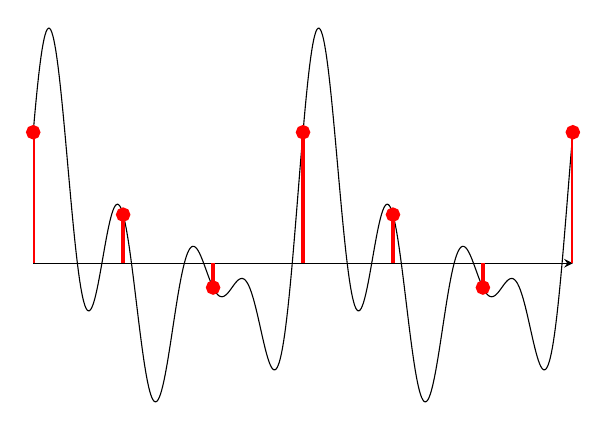
\begin{tikzpicture}
    \begin{axis}[
        domain=-360:360,
        samples=501,
        xtick=\empty,
        ytick=\empty,
        axis y line=none,
        axis x line=middle,
      ]
      \plot [black] {
          0.514401*sin(x) + 0.865727*sin(2*x) + 0.421716*sin(3*x) + 0.972894*sin(4*x)
        + 0.902356*cos(x) + 0.231517*cos(2*x) + 0.764521*cos(3*x) + 0.0360703*cos(4*x)
        };
      \addplot [
          ycomb,
          mark=*,
          very thick,
          red,
          samples at={-360, -240, ..., 360}
        ] {
          0.514401*sin(x) + 0.865727*sin(2*x) + 0.421716*sin(3*x) + 0.972894*sin(4*x)
        + 0.902356*cos(x) + 0.231517*cos(2*x) + 0.764521*cos(3*x) + 0.0360703*cos(4*x)
      };
    \end{axis}
  \end{tikzpicture}
  \caption{Illustration of issues that arise due the finite number of sampels in
    a \gls{DFT}.  The samples in red are unable to encode some of the high
    frequency information.}
  \label{fig:dft}
\end{figure}

Since \(f_{\text{max}}\) is known, then it doesn't make sense to talk about the
Fourier series beyond this frequency:
\begin{equation}
  \label{eq:computer_sum}
  g(t_{i}) = \sum_{-f_{\text{max}}}^{f_{\text{max}}} \hat g(f_{n}) e^{2\pi i f_{n} t_{i}}
\end{equation}
For similar reasons, there is also a minimum frequency whose wavelength must
correspond to the full length of the time sample, and for every other
subdivision of the samples, it is possible to extract an associated frequency
\(f_{n}\).  In other words:
\begin{equation}
  f_{n} \defeq \frac{n}{N} f_{\text{max}}
\end{equation}
For \(n = 0\), then \(f_{0}\) is undefined and looks to be infinite which
actually corresponds to having a constant.

When working with discrete Fourier transforms in computing, the different
frequencies are stored in a list.  Based on the way frequencies are summed in
\cref{eq:computer_sum}, it seems sensible to sort list the frequencies as
\begin{equation}
  \left[
    f_{-N/2},
    \dots,
    f_{-2},
    f_{-1},
    f_{0},
    f_{1},
    f_{2},
    \dots,
    f_{N/2}
  \right],
\end{equation}
However, this proves to be quite inconvenient since getting the 0th frequency
requires finding the middle of the array, the 1st positive frequency is one
element after the middle, etc.  As a result, the frequencies are often stored
as:
\begin{equation}
  \left[
    f_{0},
    f_{1},
    f_{2},
    \dots,
    f_{N/2},
    f_{-N/2},
    \dots,
    f_{-2},
    f_{-1}
  \right],
\end{equation}
where the \(-1\)th frequency is the first element starting from the end, etc.

Lastly, you'll notice that the common factor of \(f_{\text{max}}\) is
superfluous and doesn't need to be carried everywhere.  Similarly, the algorithm
to calculate \(\hat g(f_{i})\) doesn't care whether \(\Delta t\) was
\SI{1}{\milli\second} or \SI{3}{\centi\metre}.  For this reason, \gls{DFT}
algorithms usually is normalized with factor of \(N\).  Furthermore, just like
different Fourier transform conventions will include normalization factor of
\(2\pi\) in different places, the \gls{DFT} normalization factors of \(N\) will
change too.  As with the Fourier transform, the convention used is unimportant
as long as it remains consistent.

\subsubsection{Fast Fourier Transforms}
\label{subsubsec:fast_fourier_transforms}

The \gls{FFT} is, as the name suggests, a way of calculating a \gls{DFT} a lot
faster.  In the naive approach of calculating a \gls{DFT}, each of the \(N\)
\(\hat g(f_{i})\) require accessing all \(N\) \(g(t_{i})\) and as a result it
takes \(\calO(N^{2})\) to calculate the \gls{DFT}.  If \(N = 100\), this is not
an issue for a computer, but if \(N = 10^{6}\), calculating a \gls{DFT} can
quickly become intractable.

A \gls{FFT} utilizes some clever tricks which exploit periodicity of the basis
functions in order to reduce some redundant calculations.  The resulting
complexity of the \gls{DFT} in order \(\calO(N \log N)\).  This may not seem
significant, but for an array of \(10^{6}\) elements, the computation time will
go from \(10^{12}\) arbitrary units to just \(1.4 \cdot 10^{7}\).  This is a
speed improvement of five orders of magnitude!  In order words, if this
\gls{FFT} computation took 1 second to compute, the naive \gls{DFT} would have
taken about 1 day to compute.

\section{Interpolating Functions}
\label{sec:interpolating_functions}

In this lab, we have to change between coordinate systems quite frequently:
\begin{equation}
  (x, y) \leftrightarrow (\xi, \eta) \leftrightarrow (\xi, \theta).
\end{equation}
In theory, when everything is over \(\bbR^{2}\), these changes of coordinates
are easy to handle; however in practice, \(p_{\theta}(\xi)\) is only known for a
finite set of \(\theta\) and \(\xi\).  Similarly, \(\mu(x, y)\) needs to be
reconstructed for a set of \(x\) and \(y\) values.  The problem is that a
particular point \((x_{i}, y_{i})\) will generally fall in between values of
\((\xi, \theta)\) as illustrated in \cref{fig:interpolation}.

\begin{figure}
  \centering
  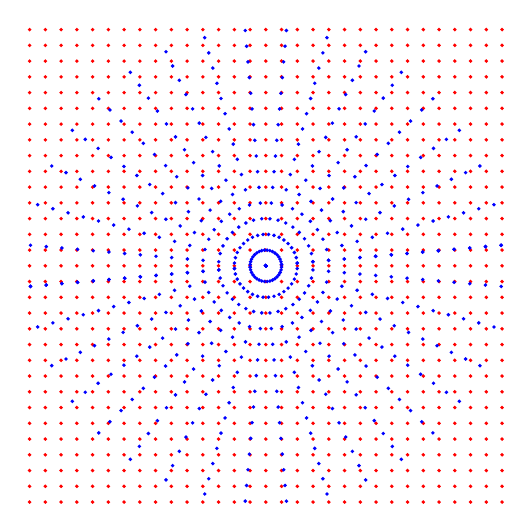
\begin{tikzpicture}
    \foreach \x in {-3, -2.8, ..., 3} {
      \foreach \y in {-3, -2.8, ..., 3} {
        \fill [red] (\x, \y) circle [radius=0.7pt];
      }
    }
    \foreach \r in {-3, -2.8, ..., 3} {
      \foreach \t in {5, 15, ..., 185} {
        \fill [blue] (\t:\r) circle [radius=0.7pt];
      }
    }
  \end{tikzpicture}
  \caption{The set of points in \((x, y)\) coordinates does not, in general,
    correspond to a nice set of points in \((\xi, \theta)\) coordinates.}
  \label{fig:interpolation}
\end{figure}

In order to fix this issue, a way to \enquote{fill in the gap} must be created
and there are several methods available.  They are explained below in terms of
\textsc{1d} problem, but they can be all generalized into \textsc{2d}
dimensions:
\begin{description}
\item[Nearest Neighbour] Use the value of the closest point that is defined:
  \begin{equation}
    \tilde f(x) = f(x_{i}) \text{ where } \abs{x_{i} - x} \text{ is minimized}
  \end{equation}
\item[Linear Interpolation] Connect known points with straight lines:
  \begin{equation}
    \tilde f(x) = \frac{f(x_{i+1}) - f(x_{i})}{x_{i+1} - x_{i}} (x - x_{i}) + f(x_{i})
  \end{equation}
\item[Cubic Spline] A \emph{spline} is a (smooth) piecewise polynomial.  The
  polynomial is define by:
  \begin{align}
    \MoveEqLeft \tilde f(t) = \left( 2t^{3} + 3t^{2} + 1 \right) f(x_{i})
    + \left( t^{3} -2t^{3} + t \right) f'(x_{i}) \\
    &+ \left( -2t^{3} + 3t^{2} \right) f(x_{i+1})
    + \left( t^{3} - t^{2} \right) f'(x_{i+1})
  \end{align}
  where \(t\) is the normalized distance between \(x_{i}\) and \(x_{i+1}\):
  \begin{equation}
    t(x) \defeq \frac{x - x_{i}}{x_{i+1} - x_{i}}.
  \end{equation}
  This requires knowledge of the derivative of \(f\) which can be computed by
  looking at points around:
  \begin{equation}
    f'(x_{i}) \approx \frac{1}{2} \frac{f(x_{i+1}) - f(x_{i})}{x_{i+1} - x_{i}}
    + \frac{1}{2} \frac{f(x_{i}) - \frac{1}{2} f(x_{i-1})}{x_{i} - x_{i-1}}
  \end{equation}
\item[Polynomial Interpolation] Given a polynomial of the form
  \begin{equation}
    p(x) = p_{n} x^{n} + p_{n-1} x^{n-1} + \dots + p_{0}
  \end{equation}
  and set of \(n\) points \(p(x_{i}) = y_{i}\), then we can form the system of
  linear equations
  \begin{equation}
    \pmtx{
      x_{0}^{n} & x_{0}^{n-1} & \dots & x_{0} & 1 \\
      x_{1}^{n} & x_{1}^{n-1} & \dots & x_{1} & 1 \\
      \vdots   & \vdots    & \ddots& \vdots & \vdots \\
      x_{n}^{n} & x_{n}^{n-1} & \dots & x_{n} & 1
    }
    \pmtx{ p_{n} \\ p_{n-1} \\ \vdots \\ p_{0} }
    =
    \pmtx{ y_{n} \\ y_{n-1} \\ \vdots \\ y_{0} }
  \end{equation}
  which can be easily solved (by a computer) for \(p_{i}\).  This then defines
  the polynomial \(p(x)\) that goes through each point \(p(x_{i}) = y_{i}\).
\end{description}

\cleardoublepage
\printbibliography

\end{document}